% This is samplepaper.tex, a sample chapter demonstrating the
% LLNCS macro package for Springer Computer Science proceedings;
% Version 2.20 of 2017/10/04
%
\documentclass[runningheads]{llncs}
%
\usepackage{amssymb}
\usepackage{amsmath}
\usepackage{graphicx}
\usepackage[misc]{ifsym} 
% Used for displaying a sample figure. If possible, figure files should
% be included in EPS format.
%
% If you use the hyperref package, please uncomment the following line
% to display URLs in blue roman font according to Springer's eBook style:
% \renewcommand\UrlFont{\color{blue}\rmfamily}

\begin{document}
%
\title{Sequence-based Recommendation with Bidirectional LSTM Network}
%
\titlerunning{Sequence-based Recommendation with Bidirectional LSTM Network}
% If the paper title is too long for the running head, you can set
% an abbreviated paper title here
%
\author{Hailin Fu \and Jianguo Li\textsuperscript{(\Letter)} \and Jiemin Chen \and Yong Tang \and Jia Zhu}
%
\authorrunning{H. Fu et al.}
% First names are abbreviated in the running head.
% If there are more than two authors, 'et al.' is used.
%
\institute{School of Computer Science, South China Normal University, \\ GuangZhou, China, 510000 \\
\email{\{hailin,jianguoli,chenjiemin,ytang,jzhu\}@m.scnu.edu.cn}}
%
\maketitle              % typeset the header of the contribution
%
\begin{abstract}
In modern recommendation systems, most methods often neglect the sequential relationship between items. So we propose a novel Sequence-based Recommendation model with Bidirectional  Long Short-Term Memory neural network (BiLSTM4Rec) which can capture the sequential feature of items to predict what a user will choose next. By collecting consumed items of a user in a sequence with time ascending order, fitting the model with the last item as the label, the rest items as the features, we regard this recommendation assignment as a super multiple classification task. Once trained well, the output layer of our model will export the probabilities of the next items with given sequence. In the experiments, we compare our approach with several commonly used recommendation methods on a real-world dataset. Experimental results indicate that our sequence-based recommender can perform well for short-term interest prediction on a sparse, large dataset.

\keywords{Recommendation system \and Social media data mining \and Sequential prediction\and Bidirectional recurrent reural network \and Deep learning.}
\end{abstract}
% 
%
%
\section{Introduction}

The primary assignments of recommendation systems faced with consist of two parts: ratings predicting and products recommendation. So to predict what a user will choose next given his consumed history is one of the crucial mission \cite{Wan2015NextBR} in recommendation area. In many websites and applications, such as online electronic business, news/videos website, music/radio station, they need an excellent service for users to recommend what they will like in future. Existing recommenders mainly concentrate on finding the neighbor sets for users or items, or leveraging other explicit/implicit information (such as tags, reviews, item contents and user profiles) for neighborhood-aware. However, to the best of our knowledge, few works use the sequential feature of data to build recommender. We find that the sequence of data implicates much exciting and relevant information, for example in a video website, the user who watched "Winter is coming" (S01, E02 of Game of Thrones) will be more likely to watch "The Kingsroad" (S01, E02 of Game of Thrones). Even at the 2011 Recsys conference, Pandora\footnote{\url{www.pandora.com}}'s researchers gave a speech about music recommendation and said they found many users consumed music in sequences.

Our work was inspired by the previous study of Siwei Lai et al. \cite{AAAI159745}, where a neural network is proposed to capture the sequence of words in a sentence.  We took a similar approach by considering one item as a word, the catalog of items as a vocabulary, and the historical consumed items of one user as a sentence, to capture the sequence of the user consumed items. The main contributions of our work are as follows:
 \begin{itemize}

\item We propose a novel Sequence-based Recommendation model with Bidirectional Long Short-Term Memory neural network,  or BiLSTM4Rec for short, which can capture the sequential features of data, as well scales linearly with the number of objectives (both of users and items).
\item We regard item sequence as a sentence and use an $M\times d$ embedding matrix $E$ to represent $M$ items which reduces memory cost evidently when faced big data.
 \end{itemize}

% The reset of the paper is organized as follows. Related work is discussed briefly in Section 2. In Section 3, we introduce the overall recommendation framework in detail. Section 4 introduces the experiments, we compare our proposed method with the traditional recommendation methods on the same real-world dataset. Finally we conclude this paper in Section 5, and point out some future work.

\section{Related Work}
\subsection{Traditional methods in recommendation}

There are three main classes of traditional recommendation systems. Those are collaborative filtering systems, content-based filtering systems, and hybrid recommendation systems \cite{1423975}. Collaborative filtering(CF) can be generally classified into Memory-based \cite{Resnick:1994:GOA:192844.192905,sarwar2001item} CF and Model-based \cite{chien1999bayesian,ungar1998clustering,mnih2008probabilistic} CF. Memory-based CF \cite{Resnick:1994:GOA:192844.192905,sarwar2001item,chien1999bayesian,ungar1998clustering} systems generate recommendations for users by finding similar user or item groups. Model-based CF systems , \emph{e.\,g.}, Bayesian networks \cite{chien1999bayesian}, clustering models \cite{ungar1998clustering}, Probabilistic Matrix Factorization \cite{mnih2008probabilistic}, mainly use the rating information to train corresponding model then use this model to predict unknown data. Content-based systems \cite{balabanovic1997fab} generate recommendations for users based on a description of the item and a profile of the user's preference. Hybrid recommendation systems \cite{burke2002hybrid} combine both collaborative and content-based approaches. However, above traditional methods are not suitable for sequential features capturing. Association rules, \emph{e.\,g.}, Apriori \cite{agrawal1993mining} and FP-Growth \cite{li2008pfp}, can be used to mine sequential features, but they suffer from sensitivity to threshold settings, high time and space complexity, missing of minority rules.

\subsection{Deep learning in recommendation}
Deep learning can efficiently capture unstructured data, and extract more complex abstractions into higher-level data representation \cite{Zhang2017DeepLB}.  Shumpei et al. \cite{okura2017embedding} presented a Recurrent Neural Network(RNN) based news recommender system for Yahoo News. Covington et al. \cite{covington2016deep} used historical query, demographic and other contextual information as features, presented a deep neural network based recommendation algorithm for video recommendation on YouTube. Hidasi, Balázs, et al. \cite{DBLP:journals/corr/HidasiKBT15} presented a Session-based recommendation with an RNN variant, i.e., GRU. Wan, Shengxian, et al. \cite{Wan2015NextBR} also used RNN to build a next basket recommendation. Zhu Y et al. \cite{ijcai2017-504} used a LSTM variant, i.e., Time-LSTM, to model users’ sequential actions. Tang et al. \cite{Tang:2018:PTS:3159652.3159656} propose Convolutional Sequence Embedding Recommendation Model which incorporates the Convolutional Neural Network (CNN) to learn sequential features, and Latent Factor Model (LFM) to learn user specific features to personalized top-N sequential recommendation. Those works show deep neural networks suit recommendation and RNN architectures are good at modeling the sequential order of objects.

\section{Proposed Approach}

We propose a novel deep neural model to capture the sequence feature of the user's consumed data. Our model mainly consists of five layers: embedding, recurrent structure, fully-connected layer, pooling layer and output layers. Figure 1 shows the structure of our sequence-based recommender.
\begin{figure}[htbp]
\centerline
{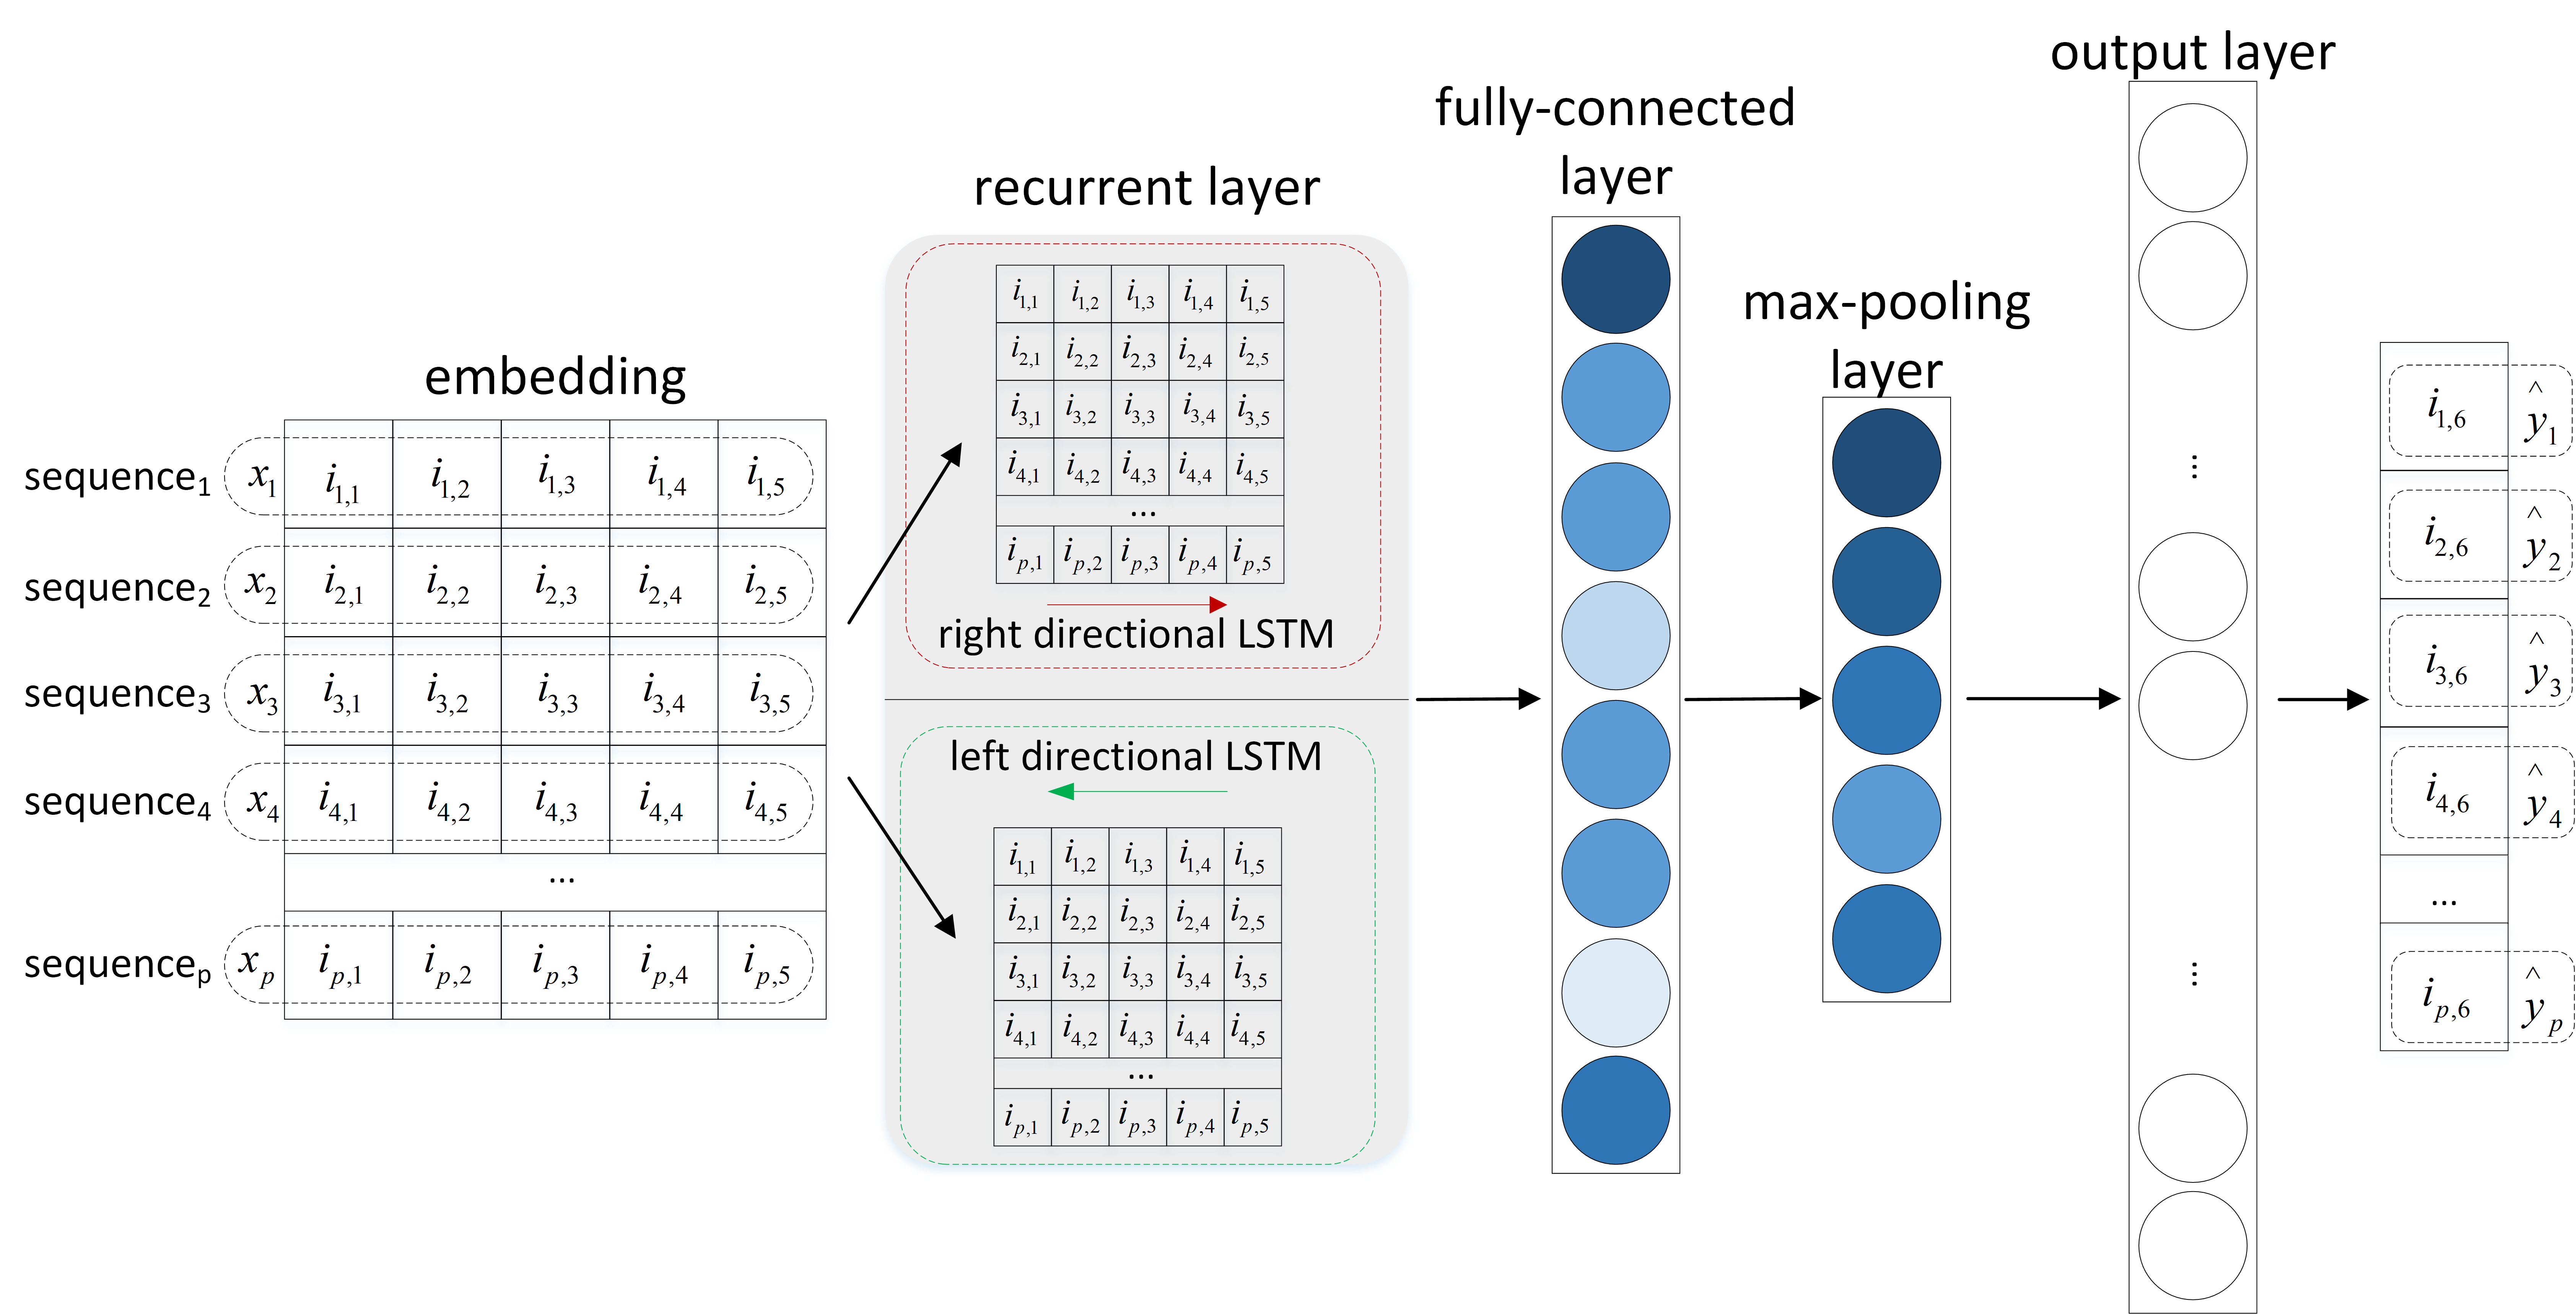
\includegraphics[height=6.2cm,width=\linewidth]{image/structer.png}}
\caption{Framework of sequence-based recommendation }
% \label{fig}
\end{figure}
\subsection{Notations }\label{AA}
Let us assume that $\mathbb{U}= \left \{ u_{1},u_{2},...,u_{N} \right \}\label{eq}$ is the user set and $\mathbb{I}= \left \{ i_{1},i_{2},...,i_{M} \right \}$ is the item set. For each user $u$, there is an observed consumed items sequence $\mathbb{S}_{u}=\left \{ s_{u}^{1},s_{u}^{2},...,s_{u}^{t-1},s_{u}^{t} \right \}$ in ascending order of time, where $s_{u}^{t}$ is the item consumed by user $u$ at time $t$. The sequential prediction problem is to predict $s_{u}^{t+1}$ for each user $u$.

We consider any item can appear only once in the history of a user. Therefore model could recommend items that the user had not yet selected. The output of the network is a softmax layer with a neuron mapping an item in the catalog. We use $p(i_{k}|S_{u},\theta )$ to represent the probability that user $u$ who had a historical consumed items sequence $S_{u}$ would select item $i_{k}$ at next time, where $\theta$ is the parameters in the network.

\subsection{Embedding layer}
 We use the latest sequences of user consumed items as the features, and the last item as the label, to build a super multiple classification supervised learning model. So in the period of the feature engineering, we need to convert the features into vectors and map them with labels. One-hot vector representation is the most common method to discrete every item. However, One-hot encoded vectors are high-dimensional and sparse. If we use One-hot encoding to deal with 1000 items, each item will be represented by a vector containing 1000 integers, 999 of which are zeros. In a big dataset, this approach is unacceptable considering computational efficiency. Word Embedding shines in the field of Natural Language Processing, instead of ending up with huge One-hot encoded vectors we also can use an embedding matrix to keep the size of each vector much smaller:
 \begin{equation}
e(I_{i})=EI_{i}
\end{equation}
where $E\in \mathbb{R}^{|e|\times |M|}$, $|e|$ is the size of the embedding layer, $|M|$ is the number of items in the training set. So $e(I_{i})$ is the embedding of consumed item $I_{i}$, which is a dense vector with $|e|$ real value elements.
Compared with the One-hot encoder (size of $|M|\times|M|$), our item sequence embedding matrix (size of $|e|\times|M|$) reduces memory cost rapidly when dealt with big data.

\subsection{User Short-term Interest Learning}
We combine a user consumed item $I_{u}^{t}$ and other items previous and subsequent $I_{u}^{t}$ to present the current interest of user $u$ at time $t$. The behavior sequences help us to indicate a more precise short-term interest of user. In this recommender, we use a recurrent structure, which is a bidirectional Long Short-Term Memory neural network, to capture the short-term interest of the user.

We define $h_{b}(I_{i})$ as the user's interest before consuming an item $I_{i}$ and $h_{a}(I_{i})$ as the user's interest after consuming an item $I_{i}$. Both $h_{b}(I_{i})$ and $h_{a}(I_{i})$ are dense vectors with $|h|$ real value elements. The interest $h_{b}(I_{i})$ before item $I_{i}$ is calculated using Equation (1). $W^{(b)}$ is a matrix that transforms the hidden layer (interest) into the next hidden layer. $W^{(cb)}$ is a matrix that is used to combine the interest of the current item with the next item's previous interest. $\sigma $ is a non-linear activation function. The interest $h_{a}(I_{i})$ after consuming item $I_{i}$ is calculated in a similar equation. Any user's initial interest uses the same shared parameters $h_{b}(I_{1})$. The subsequent interest of the last item in a user's history share the parameters $h_{a}(I_{n})$.
\begin{equation}
h_{b}(I_{i})=\sigma (W^{(b)}h_{b}(I_{i-1})+W^{(cb)}e(I_{i-1}))
\end{equation}
\begin{equation}
h_{a}(I_{i})=\sigma (W^{(a)}h_{a}(I_{i+1})+W^{(ca)}e(I_{i+1}))
\end{equation}
where the initial interest $h_{b}(I_{1}),h_{a}(I_{n})\in \mathbb{R}^{|h|}$, $W^{(b)},W^{(a)}\in \mathbb{R}^{|h|\times |h|}$, $W^{(cb)},W^{(ca)}\in \mathbb{R}^{|e|\times |h|}$.

As shown in Equation (2) and (3), the interest vector captures the interest in user's previous and subsequent behavior. We define the temporary status of the interest when a user takes a behavior $I_{i}$ as the Equation (4) shown. This manner concatenates the previous temporary status of interest $h_{b}(I_{i})$ before user consuming item $I_{i}$, the embedding of behavior $I_{i}$ consumed item $e(I_{i})$, and the subsequent temporary status of interest $h_{a}(I_{i})$ after user consuming item $I_{i}$.
\begin{equation}
x_{i}=[h_{b}(I_{i});e(I_{i});h_{a}(I_{i})]
\end{equation}
So using the consumed behavior sequences $\left \{ i_{1},i_{2},...,i_{n-1},i_{n} \right \}$, if our model learned the temporary interest status $x_{n-1}$, users who consumed item $i_{n-1}$ would have a bigger probability to get a recommended item $i_{n}$. The recurrent structure can obtain all $h_{b}$ in a forward scan of the consumed items sequences and $h_{a}$ in a backward scan of the consumed items sequences. After we obtain the representation $x_{i}$ of the temporary status of interest when user taking an item $I_{i}$, we apply a linear translation together with the $tanh$ activation function to $x_{i}$ and send the result to the next layer.
\begin{equation}
y_{i}^{(2)}=tanh(W^{(2)}x_{i}+b^{(2)})
\end{equation}
where $W^{(2)}\in \mathbb{R}^{H\times (|e|+2|h|)}$, $b^{(2)}\in \mathbb{R}^{H}$ are parameters to be learned, $H$ is the recurrent layer size, $y_{i}^{(2)}$ is a latent interest vector, in which each interest factor will be analyzed to determine the most useful factor for representing the users consumed items sequences.

\subsection{Popularity Trend Learning}
When all of the sequences of user's consumed items calculated, we apply a max-pooling layer.
\begin{equation}
y^{(3)}=\max_{i=1}^{n}y_{i}^{(2)}
\end{equation}
Max pooling is done by applying a max filter to non-overlapping subregions of the upper representation. With the pooling layer, the number of parameters or weights within the model reduced rapidly, which could reduce the spatial dimension of the upper input volume drastically and lessen the computation cost. We could capture the attribute throughout the entire sequence and find the most popular sequences combination in the whole users' history using the max-pooling layer. The last part of our model is an output layer as follows:

\begin{equation}
y^{(4)}=W^{(4)}y^{(3)}+b^{(4)}
\end{equation}
where $W^{(4)}\in \mathbb{R}^{O\times H}$, $b^{(4)}\in \mathbb{R}^{O}$ are parameters to be learned, $O$ is the fully-connected layer size.

Finally, a softmax activation function applied to $y^{(4)}$, which can convert the output values to the probabilities of next items. 

\begin{equation}
p_{i}= \frac{e^{y_{i}^{(4)}}}{\sum_{k=1}^{n}e^{y_{k}^{(4)}}}
\end{equation}

% \begin{figure}[htbp]
% \centerline{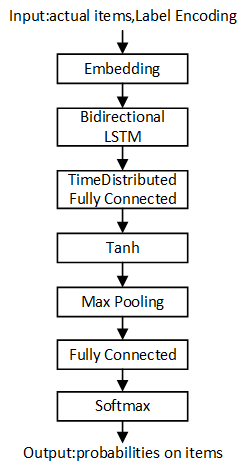
\includegraphics[width=3.5cm,height=6.5cm]{image/model.png}}
% \caption{Illustration of model structure.}
% \label{fig}
% \end{figure}
\subsection{Training}

We define all of the parameters to be trained as $\theta $.
\begin{equation}
\theta=  \left \{ E,b^{(2)},b^{(4)},h_{b}(B_{1}),h_{a}(B_{n}),W^{(2)}, W^{(4)},\right.\\
\left.W^{(b)},W^{(a)},W^{(b)},W^{(cb)},W^{(ca)} \right \} \\
\end{equation}
The training target of the network is to minimize the categorical cross entropy loss:
\begin{equation}
\mathcal{L}(y,S,\theta )=-\sum_{u\in \mathbb{U}}[y_{u}\log p(y_{u}|S_{u},\theta)+(1-y_{u})\log (1-p(y_{u}|S_{u},\theta ))]
\end{equation}
\subsection{Time Complexity Analysis}

In the embedding layer, it has a matrix multiplication operation with time complexity of $O(n)$. In the recurrent structure, for every sequence, the Bi-directional LSTM structure will apply a forward and a backward scan, and based on the citation \cite{Sak2014Long}, the time complexity of the BiLSTM we can know is $O(n)$. The time complexity of the pooling layer and the fully-connected layer is also $O(n)$. The overall model is a cascade of those layers, therefore, our sequence-based recommendation model appears a time complexity of $O(n)$, which is linearly correlated with the number of sequences. The overall time complexity of the model is more acceptable than collaborative filtering($O(n^{2})$)\cite{Resnick:1994:GOA:192844.192905,sarwar2001item}, so that big data can be effectively processed.


\section{Experiments}

\subsection{Evaluation and Metrics}

As a recommendation model, we will recommend top N item(s) for each user, denoted as $\hat{I}_{u}^{t+1}$. We adopt $Precision@N$, $Recall@N$ scores to evaluate our model and baseline models. We can define the measures as following equations:

\begin{equation}
Precision@N=\frac{\sum_{u}|\hat{I}_{u}^{t+1}\cap I_{u}^{t+1} |}{\left | \mathbb{U} \right |*N}
\end{equation}

\begin{equation}
Recall@N=\frac{\sum_{u}|\hat{I}_{u}^{t+1}\cap I_{u}^{t+1} |}{\left |\sum_{u}|I_{u}^{t+1}| \right |}
\end{equation}
In order to get a harmonic average of the precise and recall, the $F1@N$ score was measured here, where a higher F1 score reaches, a more effective result gets, which is shown as Equations (13):

\begin{equation}
F1@N=\frac{2\times Precision@N\times Recall@N}{Precision@N+Recall@N}
\end{equation}
\subsection{Dataset and Experimental Settings}

Since fewer existing recommendation datasets reserve the continuity of user behavior information, to verify our approach is feasible, we perform experiments on a real-world dataset and make it public: LiveStreaming \footnote{Data is available in https://www.kaggle.com/hailinfu/livestreaming} dataset, which collected users' behavior data from a live streaming website in China. Each line in LiveStreaming records a sequence of browsed items of a user in ascending order of time.  The initial collected LiveStreaming dataset contains 1806204 lines, which means that contacts 1806204 unique users. The length of each line ranges from 1 to 1060. Total 541772 different items contained in that dataset. We remove those users who are annotated by less than 15 items then randomly select 10 thousand users as the experimental part denoted as LiveStreaming-10M. Finally, 10000 users and 12292 items contain in LiveStreaming-10M. We randomly split 80\% of this part into training set, and keep the remaining 20\% as the validation set.

Our model is implemented on Keras with TensorFlow-gpu backend, trained on a single GeForce GTX 1050 with 4 GB memory. For hyper-parameter settings, we set: embedding layer size $|e|$ = 100, recurrent layer size $H$ = 200, fully-connected layer size $O$ = 100, batch size as 32 and initial number of epochs as 100, learning rate $\alpha$ as 0.01, momentum $\beta $ as 0.9, we adopt classification top 20 accuracy as the evaluation metric.Our code is publicly available\footnote{Code is available in https://github.com/fuhailin/BiLSTM4Rec}.


% \begin{figure}[htbp]
% \centerline
% {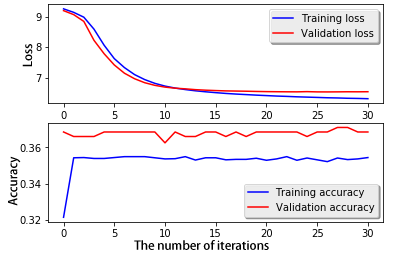
\includegraphics[height=6.2cm]{image/10thousand@6.png}}
% \caption{BiLSTM4Rec training on 80\% LiveStreaming-10M with Time Windows as 5, and recommends items with the top 20 probability values}
% \label{fig}
% \end{figure}

We also explore how many data the BiLSTM4Rec model needs for every user to learn the global sequences tendency and make a good recommendation, so we design an experiment using LiveStreaming-10M with different Time Windows ranges from 1 to 10. When Time Windows equals to 1, means we only use the last item in the sequence as label, the latest one item as feature to fit our model. Figure 3 shows that when Time Windows is less than 6, the results tend to be stable. When Time Windows is too small, much information will lose; too big, it will be hard to train the model. So we choose Time Windows as five in the next experiment.
\begin{figure}[!htb]
   \begin{minipage}{0.48\textwidth}
     \centering
     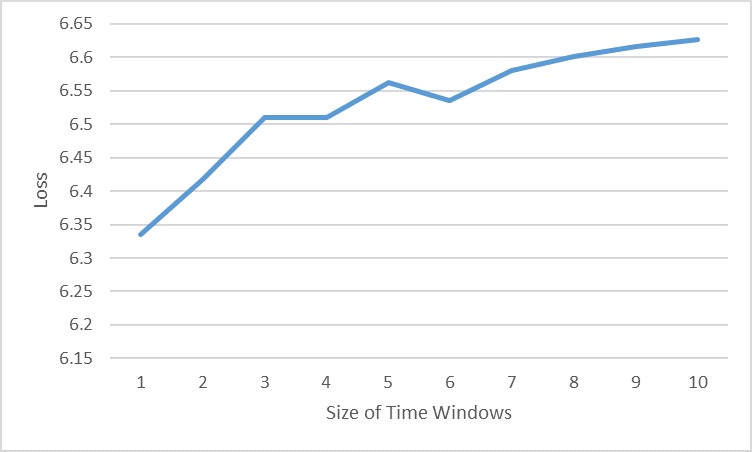
\includegraphics[width=\linewidth]{image/Loss_timewindows.png}
     % \caption{Interpolation for Data 1}
     % \label{Fig:Data1}
   \end{minipage}\hfill
   \begin {minipage}{0.48\textwidth}
     \centering
     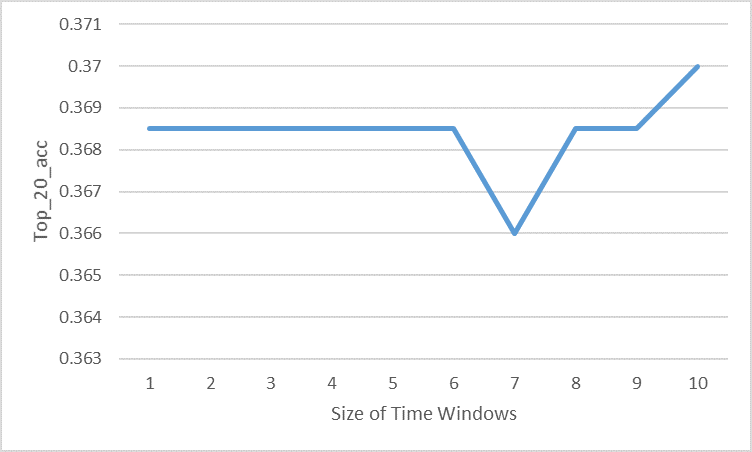
\includegraphics[width=\linewidth]{image/Top_20_acc_timewindows.png}
     % \caption{Interpolation for Data 2}
     % \label{Fig:Data2}
   \end{minipage}
   \caption{The training results of BiLSTM4Rec model on 80\% LiveStreaming-10M with different Time Windows}
   % \label{fig:coffee}
\end{figure}

\begin{figure}[!htb]
   \begin{minipage}{0.48\textwidth}
     \centering
     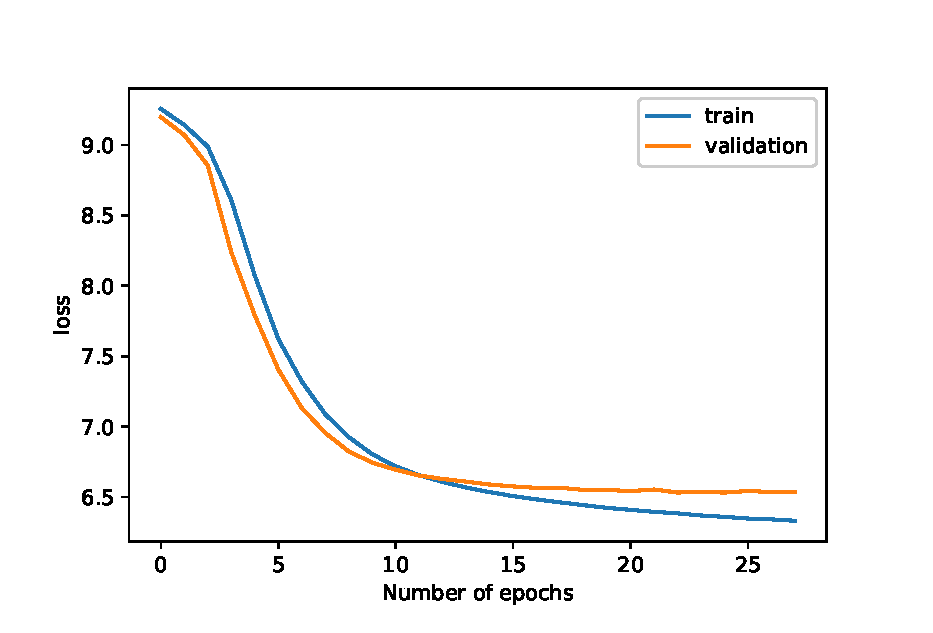
\includegraphics[width=\linewidth]{image/model_loss.eps}
     % \caption{Interpolation for Data 1}
     % \label{Fig:Data1}
   \end{minipage}\hfill
   \begin {minipage}{0.48\textwidth}
     \centering
     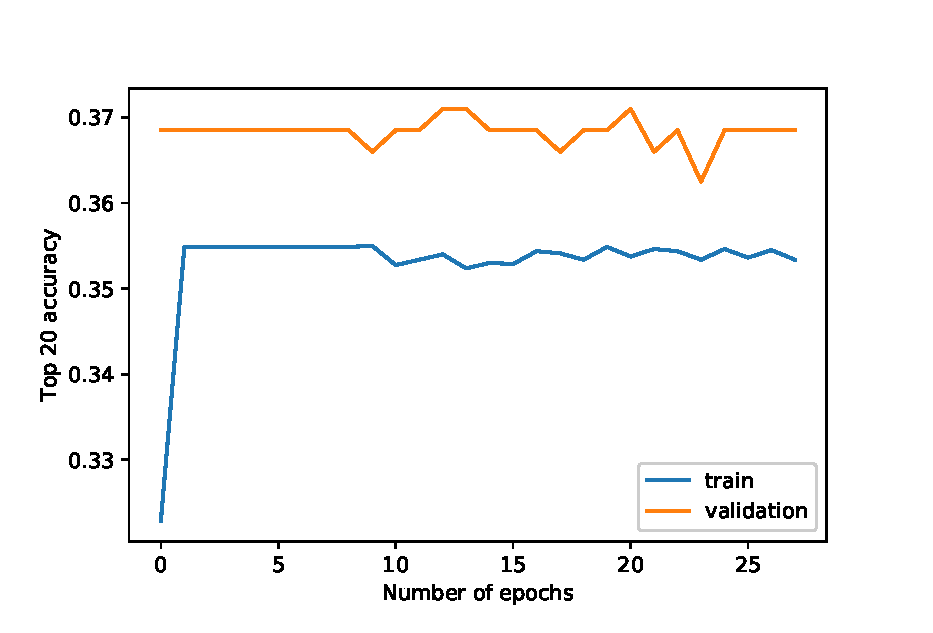
\includegraphics[width=\linewidth]{image/Top_20_accuracy.eps}
     % \caption{Interpolation for Data 2}
     % \label{Fig:Data2}
   \end{minipage}
   \caption{BiLSTM4Rec training on 80\% LiveStreaming-10M with Time Windows as 5, and recommends items with the top 20 probability values}
   % \label{fig:coffee}
\end{figure}


\subsection{Compared Algorithms}
In this paper, We compare our model with several existing baselines, and the state-of-the-art approaches in the area of recommendation system:

 \begin{itemize}
\item \textbf{POP}: Popularity predictor that always recommends the most popular items of the training set, it feedbacks the global popularity. Despite its simplicity, it is often a strong baseline in certain domains.
% \item \textbf{T-POP}: This baseline recommends the most popular items at the current moment.
\item \textbf{IBCF}:As the most classical methods of recommendation, Item-based Collaborative Filtering (IBCF) \cite{sarwar2001item}and User-based Collaborative Filtering (UBCF) \cite{Resnick:1994:GOA:192844.192905}, both yet still strong baselines for top-N recommendation. In this task, we set the rating 1 if user consumed the corresponding item, or 0 if not. Similarity between $u_{i}$ and $u_{j}$ was measured using cosine angle:
\begin{equation}
sim(u_{i},u_{j})=\cos (\vec{u_{i}},\vec{u_{j}})=\frac{\vec{u_{i}}\cdot \vec{u_{j}}}{\left \| \vec{u_{i}} \right \|_{2}\ast \left \| \vec{u_{j}} \right \|_{2}}
\end{equation}

\item \textbf{UBCF}: User-based Collaborative Filtering which evaluates the similarity between items by different users' ratings on the item, recommending items similar to those items consumed already for user. In UBCF, we also use cosine angle to measure similarity between items.

\item \textbf{LSTM}: We also compared with the basic Long Short Term Memory (LSTM) \cite{Hochreiter:1997:LSTM} model. In the embedding stage, LSTM and BiLSTM4Rec share the same size of the embedding layer. The commonly-used update equations of LSTM are as follows:
\begin{equation}
\begin{aligned}
    i_{t} & =\sigma\big(x_{t}U^{i}+h_{t-1}W^{i}\big)\\
    f_{t} & =\sigma\big(x_{t}U^{f}+h_{t-1}W^{f}\big)\\
    o_{t} & =\sigma\big(x_{t}U^{o}+h_{t-1}W^{o}\big)\\
    C_{t} & =\sigma\big(f_{t}\ast C_{t-1}+i_{t}\ast\tanh\big(x_{t}U^{g}+h_{t-1}W^{g}\big)\big)\\
    h_{t} & =\tanh(C_{t})\ast o_{t}
\end{aligned}
\end{equation}
Here, we use $i$, $f$, $o$ to denote the $input$, $forget$ and $output$ gates respectively. We also set the units of LSTM as 200.
% \item \textbf{PMF}: 
% \item \textbf{Apriori}:
\end{itemize}

\begin{table}[htbp]
\begin{center}
\begin{tabular}{|c|c|c|c|c|c|}
\hline

\textbf{Metrics}& \textbf{POP}& \textbf{UBCF}& \textbf{IBCF}& \textbf{LSTM}& \textbf{BiLSTM4Rec} \\
\hline
Precision@1& 0.0056& 0.0108 & 0.0112 & 0.1135 & \textbf{0.1165} \\
\hline
Recall@1& 0.0056& 0.0108 & 0.0112 & 0.1135 & \textbf{0.1165}\\
\hline
F1@1& 0.0056& 0.0108 & 0.0112 & 0.1135 & \textbf{0.1165}\\
\hline
Precision@5& 0.00018& 0.0476 & 0.006223 & 0.0463 & \textbf{0.0488}\\
\hline
Recall@5& 0.0009& 0.0476 & 0.0313 & 0.2315 & \textbf{0.244}\\
\hline
F1@5& 0.0003& 0.0476 & 0.010433333 & 0.077167 & \textbf{0.081333}\\
\hline
Precision@20& 0.00015& \textbf{0.1154} & 0.004705 & 0.01825 & 0.01895\\
\hline
Recall@20& 0.003& 0.1154 & 0.0941 & 0.365 & \textbf{0.379}\\
\hline
F1@20& 0.000285714& \textbf{0.1154} & 0.008961905 & 0.034762 & 0.036095\\
\hline
\end{tabular}
\label{tab1}
\end{center}
\caption{When the length of recommendation list is 1,5,20 respectively, we compare different approaches using LiveStreaming-10M dataset with Time Windows as 5}
\end{table}
Our experiments firstly compare BiLSTM4Rec model with itself in different length of sequence. From the Fig.2 we can conclude that our sequence-based recommendation also can make recommendations for someone even though with a little information about him. Furthermore, from the results (Tab. 1), we can see that the performances of our approach are better than other traditional recommendation baselines on this living broadcast dataset, especially when faced with short-term predictions. Our experiments have also demonstrated that LSTM is effective for sequence modeling, and our BiLSTM4Rec model does have a certain improvement over the basic LSTM model in the sequence based recommendation.

\section{Results and Conclusion}

Overall, BiLSTM4Rec is a novel recommendation by modeling recent consumed items as a "sentence" to predict what users will choose next. We introduced the Bidirectional Long Short-Term Memory neural network to a new application domain: recommendation system. We dealt with consumed items sequences by embedding matrix to save memory cost, and the final model can learn short-term interest of the user. Experimental results show that our approach outperforms existing methods to a great extent, and shows it is suitable to do a short-term prediction. Moreover, it doesn't have an unacceptable time complexity.

In future work, we want to use neural networks to capture other information not only the sequences of data, and to generate a more accurate and longer term prediction.

~\\
\textbf{Acknowledgement.} This work was supported by the National Natural Science Foundation of China (No. 61772211, No. 61750110516), and Science and Technology Program of Guangzhou, China (No. 201508010067).

%
% ---- Bibliography ----
%
% BibTeX users should specify bibliography style 'splncs04'.
% References will then be sorted and formatted in the correct style.
%
% \bibliographystyle{splncs04}
% \bibliography{mybibliography}
%
\bibliographystyle{splncs04}
\bibliography{references}
\end{document}
